\documentclass[11pt,a4paper,]{article}
\usepackage{lmodern}

\usepackage{amssymb,amsmath}
\usepackage{ifxetex,ifluatex}
\usepackage{fixltx2e} % provides \textsubscript
\ifnum 0\ifxetex 1\fi\ifluatex 1\fi=0 % if pdftex
  \usepackage[T1]{fontenc}
  \usepackage[utf8]{inputenc}
\else % if luatex or xelatex
  \usepackage{unicode-math}
  \defaultfontfeatures{Ligatures=TeX,Scale=MatchLowercase}
\fi
% use upquote if available, for straight quotes in verbatim environments
\IfFileExists{upquote.sty}{\usepackage{upquote}}{}
% use microtype if available
\IfFileExists{microtype.sty}{%
\usepackage[]{microtype}
\UseMicrotypeSet[protrusion]{basicmath} % disable protrusion for tt fonts
}{}
\PassOptionsToPackage{hyphens}{url} % url is loaded by hyperref
\usepackage[unicode=true]{hyperref}
\hypersetup{
            pdftitle={FFORMPP: Feature-based forecast model performance prediction},
            pdfkeywords={Time series, meta-learning, mixture autoregressive models, surface regression, M4 Competition},
            pdfborder={0 0 0},
            breaklinks=true}
\urlstyle{same}  % don't use monospace font for urls
\usepackage{geometry}
\geometry{left=2.5cm,right=2.5cm,top=2.5cm,bottom=2.5cm}
\usepackage[style=authoryear-comp,]{biblatex}
\addbibresource{references.bib}
\usepackage{longtable,booktabs}
% Fix footnotes in tables (requires footnote package)
\IfFileExists{footnote.sty}{\usepackage{footnote}\makesavenoteenv{long table}}{}
\usepackage{graphicx,grffile}
\makeatletter
\def\maxwidth{\ifdim\Gin@nat@width>\linewidth\linewidth\else\Gin@nat@width\fi}
\def\maxheight{\ifdim\Gin@nat@height>\textheight\textheight\else\Gin@nat@height\fi}
\makeatother
% Scale images if necessary, so that they will not overflow the page
% margins by default, and it is still possible to overwrite the defaults
% using explicit options in \includegraphics[width, height, ...]{}
\setkeys{Gin}{width=\maxwidth,height=\maxheight,keepaspectratio}
\IfFileExists{parskip.sty}{%
\usepackage{parskip}
}{% else
\setlength{\parindent}{0pt}
\setlength{\parskip}{6pt plus 2pt minus 1pt}
}
\setlength{\emergencystretch}{3em}  % prevent overfull lines
\providecommand{\tightlist}{%
  \setlength{\itemsep}{0pt}\setlength{\parskip}{0pt}}
\setcounter{secnumdepth}{5}

% set default figure placement to htbp
\makeatletter
\def\fps@figure{htbp}
\makeatother


\title{FFORMPP: Feature-based forecast model performance prediction}

%% MONASH STUFF

%% CAPTIONS
\RequirePackage{caption}
\DeclareCaptionStyle{italic}[justification=centering]
 {labelfont={bf},textfont={it},labelsep=colon}
\captionsetup[figure]{style=italic,format=hang,singlelinecheck=true}
\captionsetup[table]{style=italic,format=hang,singlelinecheck=true}

%% FONT
\RequirePackage{bera}
\RequirePackage{mathpazo}

%% HEADERS AND FOOTERS
\RequirePackage{fancyhdr}
\pagestyle{fancy}
\rfoot{\Large\sffamily\raisebox{-0.1cm}{\textbf{\thepage}}}
\makeatletter
\lhead{\textsf{\expandafter{\@title}}}
\makeatother
\rhead{}
\cfoot{}
\setlength{\headheight}{15pt}
\renewcommand{\headrulewidth}{0.4pt}
\renewcommand{\footrulewidth}{0.4pt}
\fancypagestyle{plain}{%
\fancyhf{} % clear all header and footer fields
\fancyfoot[C]{\sffamily\thepage} % except the center
\renewcommand{\headrulewidth}{0pt}
\renewcommand{\footrulewidth}{0pt}}

%% MATHS
\RequirePackage{bm,amsmath}
\allowdisplaybreaks

%% GRAPHICS
\RequirePackage{graphicx}
\setcounter{topnumber}{2}
\setcounter{bottomnumber}{2}
\setcounter{totalnumber}{4}
\renewcommand{\topfraction}{0.85}
\renewcommand{\bottomfraction}{0.85}
\renewcommand{\textfraction}{0.15}
\renewcommand{\floatpagefraction}{0.8}

%\RequirePackage[section]{placeins}

%% SECTION TITLES
\RequirePackage[compact,sf,bf]{titlesec}
\titleformat{\section}[block]
  {\fontsize{15}{17}\bfseries\sffamily}
  {\thesection}
  {0.4em}{}
\titleformat{\subsection}[block]
  {\fontsize{12}{14}\bfseries\sffamily}
  {\thesubsection}
  {0.4em}{}
\titlespacing{\section}{0pt}{*5}{*1}
\titlespacing{\subsection}{0pt}{*2}{*0.2}


%% TITLE PAGE
\def\Date{\number\day}
\def\Month{\ifcase\month\or
 January\or February\or March\or April\or May\or June\or
 July\or August\or September\or October\or November\or December\fi}
\def\Year{\number\year}

\makeatletter
\def\wp#1{\gdef\@wp{#1}}\def\@wp{??/??}
\def\jel#1{\gdef\@jel{#1}}\def\@jel{??}
\def\showjel{{\large\textsf{\textbf{JEL classification:}}~\@jel}}
\def\nojel{\def\showjel{}}
\def\addresses#1{\gdef\@addresses{#1}}\def\@addresses{??}
\def\cover{{\sffamily\setcounter{page}{0}
        \thispagestyle{empty}
        \placefig{2}{1.5}{width=5cm}{monash2}
        \placefig{16.9}{1.5}{width=2.1cm}{MBusSchool}
        \begin{textblock}{4}(16.9,4)ISSN 1440-771X\end{textblock}
        \begin{textblock}{7}(12.7,27.9)\hfill
        \includegraphics[height=0.7cm]{AACSB}~~~
        \includegraphics[height=0.7cm]{EQUIS}~~~
        \includegraphics[height=0.7cm]{AMBA}
        \end{textblock}
        \vspace*{2cm}
        \begin{center}\Large
        Department of Econometrics and Business Statistics\\[.5cm]
        \footnotesize http://monash.edu/business/ebs/research/publications
        \end{center}\vspace{2cm}
        \begin{center}
        \fbox{\parbox{14cm}{\begin{onehalfspace}\centering\Huge\vspace*{0.3cm}
                \textsf{\textbf{\expandafter{\@title}}}\vspace{1cm}\par
                \LARGE\@author\end{onehalfspace}
        }}
        \end{center}
        \vfill
                \begin{center}\Large
                \Month~\Year\\[1cm]
                Working Paper \@wp
        \end{center}\vspace*{2cm}}}
\def\pageone{{\sffamily\setstretch{1}%
        \thispagestyle{empty}%
        \vbox to \textheight{%
        \raggedright\baselineskip=1.2cm
     {\fontsize{24.88}{30}\sffamily\textbf{\expandafter{\@title}}}
        \vspace{2cm}\par
        \hspace{1cm}\parbox{14cm}{\sffamily\large\@addresses}\vspace{1cm}\vfill
        \hspace{1cm}{\large\Date~\Month~\Year}\\[1cm]
        \hspace{1cm}\showjel\vss}}}
\def\blindtitle{{\sffamily
     \thispagestyle{plain}\raggedright\baselineskip=1.2cm
     {\fontsize{24.88}{30}\sffamily\textbf{\expandafter{\@title}}}\vspace{1cm}\par
        }}
\def\titlepage{{\cover\newpage\pageone\newpage\blindtitle}}

\def\blind{\def\titlepage{{\blindtitle}}\let\maketitle\blindtitle}
\def\titlepageonly{\def\titlepage{{\pageone\end{document}}}}
\def\nocover{\def\titlepage{{\pageone\newpage\blindtitle}}\let\maketitle\titlepage}
\let\maketitle\titlepage
\makeatother

%% SPACING
\RequirePackage{setspace}
\spacing{1.5}

%% LINE AND PAGE BREAKING
\sloppy
\clubpenalty = 10000
\widowpenalty = 10000
\brokenpenalty = 10000
\RequirePackage{microtype}

%% PARAGRAPH BREAKS
\setlength{\parskip}{1.4ex}
\setlength{\parindent}{0em}

%% HYPERLINKS
\RequirePackage{xcolor} % Needed for links
\definecolor{darkblue}{rgb}{0,0,.6}
\RequirePackage{url}

\makeatletter
\@ifpackageloaded{hyperref}{}{\RequirePackage{hyperref}}
\makeatother
\hypersetup{
     citecolor=0 0 0,
     breaklinks=true,
     bookmarksopen=true,
     bookmarksnumbered=true,
     linkcolor=darkblue,
     urlcolor=blue,
     citecolor=darkblue,
     colorlinks=true}

%% KEYWORDS
\newenvironment{keywords}{\par\vspace{0.5cm}\noindent{\sffamily\textbf{Keywords:}}}{\vspace{0.25cm}\par\hrule\vspace{0.5cm}\par}

%% ABSTRACT
\renewenvironment{abstract}{\begin{minipage}{\textwidth}\parskip=1.4ex\noindent
\hrule\vspace{0.1cm}\par{\sffamily\textbf{\abstractname}}\newline}
  {\end{minipage}}


\usepackage[T1]{fontenc}
\usepackage[utf8]{inputenc}

\usepackage[showonlyrefs]{mathtools}
\usepackage[no-weekday]{eukdate}

%% BIBLIOGRAPHY

\makeatletter
\@ifpackageloaded{biblatex}{}{\usepackage[style=authoryear-comp, backend=biber, natbib=true]{biblatex}}
\makeatother
\ExecuteBibliographyOptions{bibencoding=utf8,minnames=1,maxnames=3, maxbibnames=99,dashed=false,terseinits=true,giveninits=true,uniquename=false,uniquelist=false,doi=false, isbn=false,url=true,sortcites=false}

\DeclareFieldFormat{url}{\texttt{\url{#1}}}
\DeclareFieldFormat[article]{pages}{#1}
\DeclareFieldFormat[inproceedings]{pages}{\lowercase{pp.}#1}
\DeclareFieldFormat[incollection]{pages}{\lowercase{pp.}#1}
\DeclareFieldFormat[article]{volume}{\mkbibbold{#1}}
\DeclareFieldFormat[article]{number}{\mkbibparens{#1}}
\DeclareFieldFormat[article]{title}{\MakeCapital{#1}}
\DeclareFieldFormat[inproceedings]{title}{#1}
\DeclareFieldFormat{shorthandwidth}{#1}
% No dot before number of articles
\usepackage{xpatch}
\xpatchbibmacro{volume+number+eid}{\setunit*{\adddot}}{}{}{}
% Remove In: for an article.
\renewbibmacro{in:}{%
  \ifentrytype{article}{}{%
  \printtext{\bibstring{in}\intitlepunct}}}

\makeatletter
\DeclareDelimFormat[cbx@textcite]{nameyeardelim}{\addspace}
\makeatother
\renewcommand*{\finalnamedelim}{%
  %\ifnumgreater{\value{liststop}}{2}{\finalandcomma}{}% there really should be no funny Oxford comma business here
  \addspace\&\space}


\wp{no/yr}
\jel{C10,C14,C22}

\RequirePackage[absolute,overlay]{textpos}
\setlength{\TPHorizModule}{1cm}
\setlength{\TPVertModule}{1cm}
\def\placefig#1#2#3#4{\begin{textblock}{.1}(#1,#2)\rlap{\includegraphics[#3]{#4}}\end{textblock}}


\nocover

\author{Thiyanga S.~Talagala, Feng~Li, Yanfei~Kang}
\addresses{\textbf{Thiyanga S. Talagala}\newline
Department of Econometrics and Business Statistics, Monash University, VIC 3800, Australia, and \newline ARC Centre of Excellence for Mathematics and Statistical Frontiers
\newline{Email: \href{mailto:thiyanga.talagala@monash.edu}{\nolinkurl{thiyanga.talagala@monash.edu}}}\newline Corresponding author\\[1cm]
\textbf{Feng Li}\newline
School of Statistics and Mathematics, Central University of Finance and Economics, Beijing 100081, China
\newline{Email: \href{mailto:feng.li@cufe.edu.cn}{\nolinkurl{feng.li@cufe.edu.cn}}}\\[1cm]
\textbf{Yanfei Kang}\newline
School of Economics and Management, Beihang University, Beijing 100191, China
\newline{Email: \href{mailto:yanfeikang@buaa.edu.cn}{\nolinkurl{yanfeikang@buaa.edu.cn}}}\\[1cm]
}

\date{\sf\Date~\Month~\Year}
\makeatletter
 \lfoot{\sf Talagala, Li, Kang: \@date}
\makeatother

%% Any special functions or other packages can be loaded here.
%% Any special functions or other packages can be loaded here.
%% Any special functions or other packages can be loaded here.
%% Any special functions or other packages can be loaded here.
%% Any special functions or other packages can be loaded here.
\usepackage{tikz}
\usepackage{algorithm}
\usepackage{algpseudocode}
\usepackage{amsthm}
\usepackage{amsmath,bm}
\usepackage{paralist}
\usepackage{todonotes}
\usepackage{ctable}
\usepackage{multirow}
\usepackage{lscape}
\usepackage{rotating}
\usepackage{float} 
\usepackage{enumitem}
\usepackage[referable]{threeparttablex}
\floatplacement{figure}{H} 

\def\sectionautorefname{Section}
\captionsetup[figure]{font=small}
\captionsetup[table]{font=small}
\def\var{\text{Var}}
\allowdisplaybreaks
\sloppy

%% LINE AND PAGE BREAKING
\clubpenalty = 4500
\widowpenalty = 4500
\brokenpenalty = 4500


\def\yes{$\checkmark$}

\setlength{\abovedisplayskip}{5pt}
\setlength{\belowdisplayskip}{5pt}
\setlength{\abovedisplayshortskip}{0pt}
\setlength{\belowdisplayshortskip}{0pt}


\begin{document}
\maketitle
\begin{abstract}
This paper introduces a novel meta-learning algorithm for time series forecasting. The efficient Bayesian multivariate surface regression approach is used to model forecast error as a function of features calculated from the time series. The minimum predicted forecast error is then used to identify an individual model or combination of models to produce forecasts. In general, the performance of any meta-learner strongly depends on the reference dataset used to train the model. We further examine the feasibility of using GRATIS (a feature-based time series simulation approach) in generating a realistic time series collection to obtain a diverse collection of time series for our reference set. The proposed framework is tested using the M4 competition data and is compared against several benchmarks and other commonly used forecasting approaches. The new approach obtains performance comparable to the second and the third rankings of the M4 competition.
\end{abstract}
\begin{keywords}
Time series, meta-learning, mixture autoregressive models, surface regression, M4 Competition
\end{keywords}

\hypertarget{intro}{%
\section{Introduction}\label{intro}}

Forecasting is an important aspect of every business operation. The selection of a suitable forecast model or a combination of models to use in forecasting is at the heart of the forecasting process \autocite{tashman1991automatic}. This selection process is challenging in the context of large-scale time series forecasting for several reasons: i) there is no universal method that performs best for all kinds of forecasting problems; ii) a trial-and-error process of model selection would increase the time and computational cost significantly; iii) it is not possible to derive a typical algebraic expression for choosing the best-performing model(s) out of a portfolio of algorithms; and iv) even with expert knowledge, the correct solution is not guaranteed. A meta-learning approach serves as a promising alternative to solve this problem.

The idea of using meta-learning to select the best forecasting model for a given time series has been explored by several researchers in the context of time series forecasting \autocites{collopy1992rule}{shah1997model}{adya2001automatic}{wang2009rule}{Petropoulos2014}. This approach is also known as an algorithm selection problem and can be expressed firmly using Rice's framework for algorithm selection \autocite{rice1976}. Further evidence in favour of this idea is also given in \textcite{fforms}. In all these cases, a vector of features computed from time series is used as input to train a meta-learner. The output and the objective function to train the meta-learner is approached differently. For example, \textcite{shah1997model} uses the best forecast model as the output label and applies a discriminant analysis to train a meta-learner to predict the forecast model that is expected to perform best on a given time series. The objective function is to minimise classification error. Further, \textcite{prudencio2004using} use neural network approaches to define weights for the best linear combination of methods to improve forecast accuracy; thus, the objective function is to minimise forecast error.

Although many researchers have highlighted the usefulness of the meta-learning approach to guide the way the forecasts are computed, few studies have concluded that this approach is superior to simple benchmarks and commonly used forecasting approaches. For example, \textcite{meade2000evidence} concludes that the summary statistics are useful in selecting a good forecasting method, but are not necessarily the best. Two possible reasons for the infeasibility of the selection process are the use of inadequate features in the meta-learning process, and having training time series data that are not as diverse as required to predict different forecast model performance \autocite{kang2019gratis}.

This paper is the third in a series of papers addressing the aforementioned issues in developing a meta-learning framework for forecast model selection based on features computed from the time series. Our first attempt to develop a framework for forecast model selection is described in \textcite{fforms}. The first framework is called FFORMS: Feature-based FORecast Model-Selection. We use the random forest algorithm to predict the forecast model that is expected to perform best on a given time series. In our second paper, \textcite{fforma}, rather than mapping time series to a single forecast model we use a gradient boosting algorithm to obtain the weights for forecast combinations. We call our second framework FFORMA: Feature-based FORecast Model Averaging. FFORMA placed second in the M4 competition \autocite{makridakis2018m4}. Having revisited the literature, we found that to the best of our knowledge none of these studies have considered the correlation structure of algorithm performance in their model training process. The current paper extends this idea. The third algorithm uses the efficient Bayesian multivariate surface regression approach to estimate forecast error for each method, and then uses the minimum predicted error to select a forecasting model or choose individual models for forecast combinations.

The main contributions of this paper are as follows:

\begin{enumerate}
\def\labelenumi{\arabic{enumi}.}
\item
  We propose a novel meta-learning framework for time series forecasting. We refer to this general framework as FFORMPP: Feature-based FORecast Model Performance Prediction. It consists
  of two phases: the offline phase and the online phase. Most of the expensive computations for processing data and training a meta-learner are performed in the offline phase. We use a collection of time series to train a meta-learner. The data processing part requires computation of a set of features and forecast errors from a pool of forecast models for the time series in our collection. Subsequently, the efficient Bayesian multivariate surface regression approach proposed by \textcite{li2013efficient} is used to model forecast algorithm performances (measured by a forecast error measure, which in our case is MASE: Mean Absolute Scaled Error) as a function of features calculated from the time series. This produces a meta-learner to be used in the online phase. The online phase requires only the calculation of a simple vector of features for any newly given time series and uses the pre-trained classifier to estimate forecast error for each model in the pool, which is computationally efficient for real-time implementations. This allows ranking of the forecast models with respect to their forecast errors and evaluation of their relative forecast performance without calculating forecasts from all available individual models in the pool.
\item
  The diversity of features in the collection of time series used to train a meta-learner plays a critical role in training a meta-learning model. Often, time series with the required amount of feature diversity and quality might not be available \autocites{kang2017visualising}{kang2019gratis}. To this end, we explore the use of GRATIS (GeneRAting TIme Series with diverse and controllable characteristics) proposed by \textcite{kang2019gratis} to obtain a diverse collection of time series.
\item
  We visualise time series in the instance space defined by the features according to the forecast models used to compute combination forecasts. This helps us to explore the distribution of locations of the time series in the instance space and their relationship with features and forecast model selection.
\end{enumerate}

The remainder of the paper is organised as follows: \autoref{methodology} introduces the methodology, including the methodology for simulating time series to augment the reference set to train a model and efficient Bayesian multivariate regression approach. \autoref{results} discusses the results in application to the M4 competition data. \autoref{conclusion} concludes the paper.

\hypertarget{methodology}{%
\section{Methodology}\label{methodology}}

\autoref{fig:framework} shows the proposed framework. For each series, a set of features computed from the training period of each series comprising an input vector and the MASE values for each method gives the output vector to train a model. The description of the features calculated in each frequency category is shown in \autoref{feature}. We analyse yearly, quarterly, monthly, weekly, daily and hourly series separately. \autoref{classlabels} shows the forecast models we consider within each frequency category.

\begin{figure}[h]

{\centering 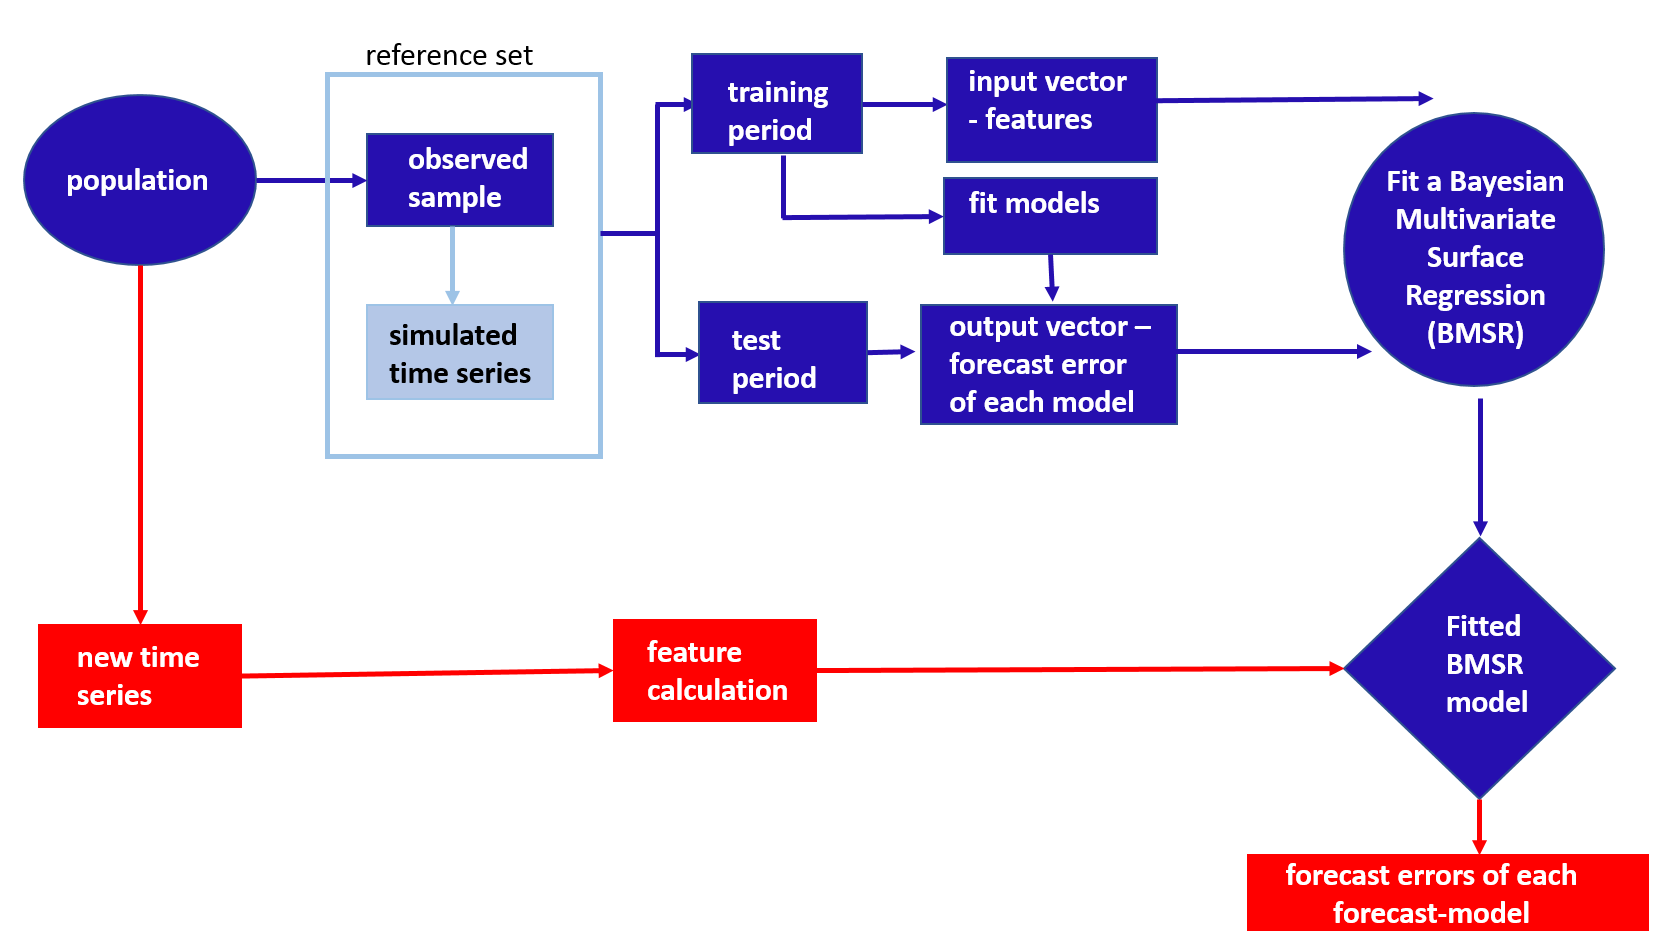
\includegraphics[width=1.05\linewidth,height=0.4\textheight]{img/frameworkfformpp} 

}

\caption{FFORMPP (Feature-based FORecast Model Performance Prediction) framework. The offline phase is shown in blue and the online phase in red.}\label{fig:framework}
\end{figure}

\begin{table}[!htp]
\centering\footnotesize\tabcolsep=0.12cm
\caption{Time series features}
\label{feature}
\begin{tabular}{llp{8,8cm}cccc}
\toprule
\multicolumn{2}{c}{Feature} & Description & Y & Q/M & W & D/H\\
\midrule
1  & T              & length of time series                                                                   & \yes  & \yes & \yes & \yes\\
2  & trend          & strength of trend                                                                       & \yes  & \yes & \yes & \yes\\
3  & seasonality\_q    & strength of quarterly seasonality                                                    & -     & \yes & - & -\\
4  & seasonality\_m    & strength of monthly seasonality                                                      & -     & \yes & - & -\\
5  & seasonality\_w    & strength of weekly seasonality                                                       & -     & - & \yes & \yes \\
6  & seasonality\_d    & strength of daily seasonality                                                        & -     & - & - & \yes\\
7  & seasonality\_y    & strength of yearly seasonality                                                       & -     & - & - & \yes\\
8  & linearity      & linearity                                                                               & \yes  & \yes & \yes & \yes\\
9  & curvature      & curvature                                                                               & \yes  & \yes & \yes & \yes\\
10  & spikiness      & spikiness                                                                               & \yes  & \yes & \yes & \yes\\
11  & e\_acf1        & first ACF value of remainder series                                                     & \yes  & \yes & \yes & \yes\\
12  & stability      & stability                                                                               & \yes  & \yes & \yes & \yes\\
13  & lumpiness      & lumpiness                                                                               & \yes  & \yes & \yes & \yes\\
14 & entropy        & spectral entropy                                                                        & \yes  & \yes & \yes & \yes\\
15 & hurst          & Hurst exponent                                                                          & \yes  & \yes & \yes & \yes\\
16 & nonlinearity   & nonlinearity                                                                            & \yes\ & \yes & \yes & \yes\\
17 & alpha          & ETS(A,A,N) $\hat\alpha$                                                                 & \yes  & \yes & \yes & -\\
18 & beta           & ETS(A,A,N) $\hat\beta$                                                                  & \yes  & \yes & \yes & - \\
19 & hwalpha        & ETS(A,A,A) $\hat\alpha$                                                                 & -     & \yes & - & -\\
20 & hwbeta         & ETS(A,A,A) $\hat\beta$                                                                  & -     & \yes & - & - \\
21 & hwgamma        & ETS(A,A,A) $\hat\gamma$                                                                 & -     & \yes & - &-\\
22 & ur\_pp         & test statistic based on Phillips-Perron test                                            & \yes  & - & - & - \\
23 & ur\_kpss       & test statistic based on KPSS test                                                       & \yes  & - & - & - \\
24 & y\_acf1        & first ACF value of the original series                                                  & \yes  & \yes & \yes & \yes\\
25 & diff1y\_acf1   & first ACF value of the differenced series                                               & \yes  & \yes & \yes & \yes\\
26 & diff2y\_acf1   & first ACF value of the twice-differenced series                                         & \yes  & \yes & \yes & \yes\\
27 & y\_acf5        & sum of squares of first 5 ACF values of original series                                 & \yes  & \yes & \yes & \yes\\
28 & diff1y\_acf5   & sum of squares of first 5 ACF values of differenced series                              & \yes  & \yes & \yes & \yes\\
29 & diff2y\_acf5   & sum of squares of first 5 ACF values of twice-differenced series                        & \yes  & \yes & \yes & \yes \\
30 & sediff\_acf1 & ACF value at the first lag of seasonally-differenced series                    & -     & \yes & \yes & \yes\\
31 & sediff\_seacf1 & ACF value at the first seasonal lag of seasonally-differenced series                    & -     & \yes & \yes & \yes\\
32 & sediff\_acf5   & sum of squares of first 5 autocorrelation coefficients of seasonally-differenced series & -     & \yes & \yes & \yes\\
33 & seas\_pacf     & partial autocorrelation coefficient at first seasonal lag & -     & \yes & \yes & \yes\\
34 & lmres\_acf1    & first ACF value of residual series of linear trend model                                & \yes  & - & - & -\\
35 & y\_pacf5       & sum of squares of first 5 PACF values of original series                                & \yes  & \yes & \yes & \yes\\
36 & diff1y\_pacf5  & sum of squares of first 5 PACF values of differenced series                             & \yes  & \yes & \yes & \yes\\
37 & diff2y\_pacf5  & sum of squares of first 5 PACF values of twice-differenced series                       & \yes  & \yes & \yes & \yes\\
\bottomrule
\end{tabular}
\end{table}

\begin{table}[!htp]
\centering\footnotesize\tabcolsep=0.12cm
\caption{Class labels}
\label{classlabels}
\begin{tabular}{llrrrr}
class label & Description & Y & Q/M & W & D/H \\ \hline
WN & white noise process & \checkmark & \checkmark & \checkmark & \checkmark \\
auto.arima & ARIMA processes & \checkmark & \checkmark & \checkmark & -\\
ets & exponential smoothing & \checkmark & \checkmark & - & - \\
rwd & random walk with drift & \checkmark & \checkmark & \checkmark & \checkmark \\
rw & random walk & \checkmark & \checkmark & \checkmark & \checkmark  \\
theta & standard theta method & \checkmark & \checkmark & \checkmark & \checkmark \\
stlar & STL-AR method & - & \checkmark & \checkmark & \checkmark \\
snaive & seasonal naive method & - & \checkmark & \checkmark & \checkmark \\
tbats & TBATS forecasting & - & \checkmark & \checkmark & \checkmark \\
nn & neural network time series forecasts & \checkmark & \checkmark & \checkmark & \checkmark \\
mstlets & multiple seasonal time series & - & - & \checkmark & \checkmark \\
mstlarima & multiple seasonal time series & - & - & - & \checkmark \\\hline
\end{tabular}
\end{table}

\hypertarget{reference-set}{%
\subsection{Reference set}\label{reference-set}}

We use the time series of M1 and M3 competitions as the observed sample for yearly, quarterly and monthly time series. In addition to the observed time series, we simulate 10, 000 time series based on MAR (Mixture AutoRegressive) models introduced by \textcite{kang2019gratis}. The observed time series and the simulated time series form the reference set to fit the model. For weekly, daily and hourly frequencies, only the simulated time series are used to create the reference set because the previous M-competitions do not contain the time series corresponding to weekly, daily and hourly frequencies. Once we have formed the reference set, we split each time series in the reference set into training period and test period. Features are calculated based on the training period of each series and the forecast error measure is calculated over the test period of each time series. \autoref{observedsample} summarises the number of time series in the reference set and the new time series in each frequency category. Note that for yearly, quarterly and monthly time series, the reference set used to train a meta-learner is much smaller than the test set evaluating the meta-learner. This is often the case when applying the meta-learner in practice during the online phase.

\begin{table}[!h]
\centering
\caption{Composition of the time series in the reference set and collection of new time series}
\label{observedsample}
\begin{tabular}{l|rrr|r}
\multirow{2}{*}{Frequency} & \multicolumn{3}{c|}{Reference set} &  New series \\ 
                  &   M1    &    M3   &    Simulated  &  M4 \\ \hline
  Yearly          &   181    &   645    &   10000   & 23000 \\
  Quarterly       &   203    &    756   &   10000   &  24000\\
  Monthly         &   617    &    1428   &  10000    &  48000\\
  Weekly          &   -    &   -    &  10000   & 359 \\
  Daily           &   -    &   -    &  10000   & 4227 \\
  Hourly          &   -    &    -   &  10000    & 414\\ \hline
\end{tabular}
\end{table}

\hypertarget{augmenting-the-observed-sample-with-simulated-time-series-from-mixture-autoregressive-models}{%
\subsection{Augmenting the observed sample with simulated time series from mixture autoregressive models}\label{augmenting-the-observed-sample-with-simulated-time-series-from-mixture-autoregressive-models}}

The reference set is augmented with simulated time series to obtain a more heterogeneous collection of time series for training a model. This helps to reduce overfitting to a relatively homogeneous set of data and increases generalisability of the model when applied to new time series with different conditions. Further, this is useful when there is no observed set of time series available to train a model in the offline phase. In this study, the simulated time series are generated based on the algorithm proposed by \textcite{kang2019gratis}, hereafter referred to as GRATIS\footnote{The R package \texttt{tsgeneration} accompanies this work and is publicly available on \url{https://github.com/ykang/tsgeneration}.}. Although there is no standard process for simulating time series, the most common approach involves simulation based on some data-generating processes (DGPs) such as exponential smoothing and ARIMA models. Instead of relying on a set of DGPs to generate time series, the GRATIS algorithm simulates time series based on a diverse set of time series features using MAR models. The algorithm can also allow a user to set controllable features for simulating time series. \autoref{marparameters} lists the choice of values for parameters used to simulate time series in each frequency category. We used frequencies 1, 4, 12 and 52 to generate yearly, quarterly, monthly and weekly series respectively. Daily and hourly time series with a long history often show multiple seasonal patterns. Hence, for daily series, frequencies were set to 7 (time-of-week pattern) and 365.25 (annual seasonality), while for hourly series frequencies were set to 24 (time-of-day pattern) and 168 (time-of-week pattern). None of the time series in our hourly test dataset are longer than 8760. Hence, time-of-year pattern (\(365\times24=8760\)) was not considered. Except for hourly series, length of the time series is randomly chosen from uniform distribution. The minimum and maximum values of the distributions are selected based on lower (Q1 - 1.5 \(\times\) IQR) and upper (Q3 + 1.5 \(\times\) IQR) edges of the box-and-whisker plots. We use the M4 competition data to compute the associated statistics for length. The corresponding distributions are shown in \autoref{fig:lengthboxplot}. The reason for this choice is that we use length of the time series as a feature in our meta-learning framework. Hence, lengths of the series in our reference set should cover all or the majority of time series we need to forecast. In practice, it might be difficult to obtain a reference set covering the whole length of the new time series for two main reasons: i) information regarding the range of length is not available at the offline stage (although, a rough idea about the distribution of the majority can be obtained); and ii) the range of length is very wide owing to `outlying' observations (for example, \autoref{fig:lengthboxplot}, quarterly and monthly series). In such circumstances, a reference set covering most of the lengths of future time series is a reasonable approach. Further, for each series we randomly select a number of mixing components from \(\{1, 2, 3, 4, 5\}\). Other parameters are set the same as those in \textcite{kang2019gratis}. Having each parameter set as in \autoref{marparameters}, we generate 10000 time series from each frequency category. This is to reduce the training time of the efficient Bayesian multivariate surface regression model while maintaining the diversity of the reference set.

\begin{table}[!h]
\centering\footnotesize\tabcolsep=0.12cm
\caption{GRATIS: Choice of values for parameters for simulating time series using MAR models}
\label{marparameters}
\begin{tabular}{llp{1.5cm}lp{1cm}lp{1cm}}
          Value        &      Parameter             & \multicolumn{2}{p{1cm}}{Description} \\ \hline
\multirow{6}{*}{frequency} & \multirow{6}{*}{seasonal period} &     yearly      &  1         \\  
                  &                   &     quarterly      &     4      \\ 
                  &                   &    monthly       &       12    \\  
                  &                   &      weekly     &       52    \\  
                  &                   &  daily         &      (7, 365)     \\  
                  &                   &    hourly       &     (24, 168)     \\ \hline
\multirow{6}{*}{length} & \multirow{6}{*}{length of time series} &   yearly        &         U(19, 75)  \\ 
                  &                   &     quarterly      &     U(24, 202)      \\  
                  &                   &     monthly      &   U(60, 660)        \\  
                  &                   &    weekly       &      U(93, 2610)     \\  
                  &                   &    daily       &    U(107, 9933)       \\  
                  &                   & \multicolumn{2}{p{5cm}}{hourly: 40.8\% with 748 length and 59.2\% with 1008 length} \\ \hline
 k                 &    number of mixing components               & \multicolumn{2}{p{5cm}}{For each series randomly chosen from $\{1, 2, 3, 4,5\}$} \\
$\alpha_k$                   &   weights of mixture components                & \multicolumn{2}{l}{$\alpha_k=\beta_k/\sum_{i=1}^{K}\beta_i$, where $\beta_i \sim U(0, 1)$} \\ 
$\theta_{ki}$  &  coefficients of the AR part & \multicolumn{2}{l}{N(0, 0.5)} \\ 
$\Theta_{kj}$ &  coefficients of the seasonal AR parts & \multicolumn{2}{l}{N(0, 0.5)} \\
$d_k$ &  number of differences in each component & \multicolumn{2}{l}{Bernoulli(0.9)} \\
$D_k$ & number of seasonal differences in each component & \multicolumn{2}{l}{Bernoulli(0.4)} \\
\hline
\end{tabular}
\end{table}

\begin{figure}
\centering
\includegraphics{FFORMPPworkingpaper_files/figure-latex/lengthboxplot-1.png}
\caption{\label{fig:lengthboxplot}Distribution of length of time series of the M4 competition across different frequency categories. The data points are shown in red. Horizontal blue solid line shows the lower and the upper whisker borders of each boxplot. Some outliers could be observed in yearly, quarterly and monthly categories. There are only two distinct levels of length for hourly series.}
\end{figure}

\hypertarget{efficient-bayesian-multivariate-surface-regression-approach}{%
\subsection{Efficient Bayesian multivariate surface regression approach}\label{efficient-bayesian-multivariate-surface-regression-approach}}

The most commonly used additive spline regression assumes additivity in the regressor; that is, \(E(y|x_1, ..., x_q)=\sum_{j=1}^{q}f_j(x_j),\) where \(f_j(x_j)\) is a spline regressor of the \(j^{th}\) regressor. Even though the assumption of additivity simplifies the model, it is quite a restrictive assumption. This problem has motivated research on surface models with interactions between regressors \autocite{li2013efficient}. \textcite{li2013efficient} proposed a general Bayesian approach for fitting surface models for a continuous multivariate response by combining additive splines and interactive splines. The proposed modelling is called efficient Bayesian multivariate surface regression.

The number of knots has an important influence in the resulting fit of spline regression: without enough knots the regression is underfitted and with too many knots it is overfitted. Choosing the locations of knots is also a challenge. This becomes even harder for surface regression than it is for additive models because any feasible set of \(q\)-dimensional knots is necessarily sparse in \(R^q\) when the number of regressors, \(q\), is moderate or large. This causes the curse of dimensionality. The most common approach used in the literature is to use a fixed set of knot locations, and most of these algorithms place the knots at the centroids of the clusters computed based on regressor observations. \textcite{li2013efficient} pointed out that this is impractical when estimating a surface with several regressors. Hence, the authors proposed a computationally efficient Markov chain Monte Carlo (MCMC) algorithm for the Gaussian multivariate surface regression to update the locations of the knots jointly. Instead of a fixed set of locations, the authors introduce `moving knots'.

The proposed Gaussian multivariate regression model can be written as follows:

\begin{equation}
  \label{eq:1}
\boldsymbol{Y=X_0B_0+{X_a}(\xi_a)B_a+{X_s}(\xi_s)B_s+E},
\end{equation}

where \(\bold{Y}\) is a matrix of \(n\) number of observations and \(p\) number of response variables. The rows of \(\bold{E}\) are error vectors assumed to be independent and identically distributed (iid) as \(N_p(0,\Sigma)\). The proposed efficient Bayesian multivariate surface regression model contains three components:

\begin{enumerate}
\def\labelenumi{\arabic{enumi}.}
\item
  \textbf{Linear component: } The linear component contains the original covariates including the constant term. This enters the model in linear form. The matrix \(\bold{X_0}\) is a \(n \times q_0\) vector in which the first column contains ones for the intercept. The corresponding regression coefficients are in \(\bold{B_o}\).
\item
  \textbf{Additive component: } The second component of the model contains additive spline basis functions of the covariates in \(\bold{X_0}\). This is represented by \(\boldsymbol{X_a(\xi_a)}\), where \(\xi_a\) represents the knots. It is important to note that the knots in the additive part of the model are scalars and this model allows an unequal number of knots for different covariates in the model. The matrix \(\bold{B_a}\) contains the regression coefficients corresponding to the additive component. The additive component of the model captures the non-linear relationship between features and response \(\bold{Y}\).
\item
  \textbf{Surface component: } The surface component of the model contains the radial basis function for capturing the remaining part of the surface and interactions. This is denoted by \(\boldsymbol{X_s(\xi_s)}\). Note that the \(\xi_s\) is a \(q_0\)-dimensional vector. The matrix \(\bold{B_s}\) contains the regression coefficients corresponding to the surface component and \(\xi_s\) represents the surface knots.
\end{enumerate}

For notational convenience Equation \eqref{eq:1} can be written as

\begin{equation} 
  \mathbf{Y}=\mathbf{XB+E},
  \label{eq:eqn2}
\end{equation}

where \(\bold{X=[X_0, X_a, X_s]}\) is the \(n \times q\) design matrix (\(q=q_0+q_a+q_s\)) and \(\bold{B=[B_0^{'}, B_a^{'}, B_s^{'}]}\). For a given set of fixed knot locations, the model in Equation \eqref{eq:1} is linear in regression parameters. The over-parameterised problem is addressed by using shrinkage priors to shrink small regression coefficients towards zero. The shrinkage parameters and knot locations of \(\xi_a\) and \(\xi_s\) are treated as unknown parameters to be estimated. \textcite{li2013efficient} proposed a computationally efficient MCMC algorithm to estimate shrinkage parameters and update the locations of the knots of additive and surface components jointly. This approach allows an unequal number of knots in the different covariates. In addition, separate shrinkage parameters for the linear, additive and surface parts of the model are allowed. Further, this approach permitted separate shrinkage parameters for the \(p\) responses within each of the three model parts. In contrast to other spline-bases models, this approach allows the knot locations to move freely in the regressor space, and thus fewer knots are usually required. The estimation and computation details can be found in \textcite{li2013efficient}.

\hypertarget{results}{%
\section{Application to the M4 competition data}\label{results}}

\hypertarget{dissimilarity-between-different-datasets}{%
\subsection{Dissimilarity between different datasets}\label{dissimilarity-between-different-datasets}}

Principal component analysis preserves the dissimilarity between widely separated data points rather than the similarity between nearby data points. This feature is useful for improved confidence in simulated series' representativeness of real time series. For example, if the simulated time series results in isolated clusters or highly dense clusters far apart from the real-world time series, it indicates a poor representation of the real data.

We use principal component analysis to visualise dissimilarity between the datasets: observed time series (M1 and M3), simulated series and new time series (M4) in the two-dimensional instance space. \textcolor{black}{The data were normalized using the z-scale transformation before applying PCA.} This also helps us to gain an idea about the global structure of the location of the different collections. The results for yearly, quarterly and monthly series are shown in \autoref{fig:pca}. We compute principal components using the time series in the reference set (observed series and simulated series) and project new series (M4) into the two-dimensional space spanned by the first two eigen vectors. The first two principal components explain 51.3\%, 48.7\% and 48.3\% of the total variation in the yearly, quarterly and monthly data. We see that the distribution of the simulated time series (represented by the dark orange dots) clearly nests and fills in the instance space. The simulated time series fills the instance space by further expanding the density range of observed time series rather than resulting in isolated clusters. This guarantees that the simulated data generated based on the GRATIS approach are actually representative of real data. Further, we can see that the projection of M4 series falls within the space created by the series in the reference set (M1, M3 and simulated). This is very important because our FFORMS framework is trained based on the series in the reference set; hence, the model is valid over the space of the reference set. A few M4 time series in the monthly frequency category fall outside the convex hull of the reference set in the first two principal components owing very high length. Note that for yearly, quarterly and monthly series the size of the M4 time series collection is much greater than the size of the corresponding collection of simulated series. For yearly and quarterly data, the number of time series in the M4 collection is about twice as large as the simulated series, and for monthly data the M4 competition collection is four times larger than the simulated series. This shows the efficiency of the GRATIS simulation approach in increasing the diversity of feature space without having many time series similar in size to the new time series collection from which we wish to produce forecasts.

\begin{figure}
\centering
\includegraphics{FFORMPPworkingpaper_files/figure-latex/pca-1.png}
\caption{\label{fig:pca}Distribution of yearly, quarterly and monthly time series on the PCA space. On each graph, dark orange represents the simulated series and purple denotes new time series (M4 data). In the first row observed time series in the reference are highlighted in light orange and light purple. PCA space is computed based on the time series in the reference set and then the M4 competition (new series) are projected into the two-dimensional PCA space. Except for a few series, the majority of new time series we need to forecast fall within the space of the reference set. Note that for yearly, quarterly and monthly series the size of the test set is much larger than the size of the corresponding reference set.}
\end{figure}

\autoref{fig:pca2} shows the principal component projections of weekly, daily and hourly time series. The first two principal components explain 48.7\%, 43.4\% and 45.4\% of the total variance of weekly, daily and hourly series. In all three frequency categories, M4-competition data fall within the feature space of simulated series. For weekly, daily and hourly frequency categories, simulated time series based on the GRATIS approach successfully fill in the space of the new time series. This shows the efficiency of the GRATIS approach in generating a realistic set of representative time series. This also shows that the GRATIS approach is a good choice to augment the reference set when only small amounts of training data are available. However, daily series of M4 competition series are clustered into a single location of the feature space. This is due to the quality issues of the M4 competition data. Daily series in the M4 competition are very similar to each other owing to data leakages. Examples of data leakage include, use of different segments of time series to create a new time series, and addition of a constant value to create new time series \autocite{ingel2019correlated}. This reveals that the GRATIS simulated-based approach can also be used to evaluate the quality issues in the data.

\begin{figure}
\centering
\includegraphics{FFORMPPworkingpaper_files/figure-latex/pca2-1.png}
\caption{\label{fig:pca2}Distribution of weekly, daily and hourly time series on the PCA space. On each graph, dark orange represents the simulated series and purple denotes new time series (M4 data). PCA space is computed based on the time series in the reference set and then the M4 competition (new series) are projected into the two-dimensional PCA space. In each frequency category, new series fall within the PCA space of reference set.}
\end{figure}

\hypertarget{coverage-analysis}{%
\subsection{Coverage analysis}\label{coverage-analysis}}

To obtain a more accurate estimate of the exact coverage of simulated data, we adapt the idea used by \textcite{kang2019gratis}. For this purpose, the t-Stochastic Neighbor Embedding (t-SNE) approach is adapted. The t-SNE is a non-linear dimension reduction technique that seeks to find a low-dimensional sub-manifold that preserves the local structure of the dataset. In other words, the t-SNE approach keeps the neighbouring points in the original data space close in the embedding space. To quantify the miscoverage, first a grid of 900 squares was superimposed on the region of space covered by each scatter plot shown in \autoref{fig:tsneplots}. Then the miscoverage of dataset A over dataset B is computed as follows \autocite{kang2019gratis}:

\[miscoverage_{A/B}=N^{-2}\sum_{i=1}^{N^2}(1-I_{i,A}) \times I_{i,B},\] where \(I_{i, A}= 1\) if points in dataset A fall within \(i^{th}\) square and \(I_{i, A}= 0\) otherwise. An analogous definition is applied to \(I_{i,B}\) computed based on the dataset B. We computed miscoverage of the simulated dataset over the M4 dataset and vice versa. The results are shown in \autoref{miscoverage}. \autoref{miscoverage} shows that our attempt to increase the diversity of the reference set using the GRATIS approach is successful.

\begin{figure}
\centering
\includegraphics{FFORMPPworkingpaper_files/figure-latex/tsneplots-1.png}
\caption{\label{fig:tsneplots}Two-dimensional t-SNE instance spaces of the M1, M3, M4 and simulated series for yearly, quarterly, monthly, weekly, daily and hourly series.}
\end{figure}

\begin{table}[!h]
\caption{Coverage analysis}
\label{miscoverage}
\begin{tabular}{p{5cm}rrrrrr}
\hline
 & Yearly & Quarterly & Monthly & Weekly & Daily & Hourly \\ \hline
Miscoverage of the 'Simulated' dataset over the 'M4' dataset & 0.068 & 0.043 & 0.132 & 0.001 & 0.061 & 0.011\\ \hline
Miscoverage of the 'M4' dataset over the 'Simulated' dataset  & 0.026 & 0.022 & 0.011 & 0.438 & 0.278 & 0.490 \\ \hline
\end{tabular}
\end{table}

\hypertarget{forecasting-results}{%
\subsection{Forecasting results}\label{forecasting-results}}

We evaluate the out-of-sample performances of our proposed meta-learning framework to the benchmark based on the M4 competition series. The mean absolute scale error (MASE) \autocite{hyndman2006another} was used to evaluate forecast accuracy. We compute both individual and combination forecasts for the M4 competition series. Individual forecasts are computed based on the model corresponding to the minimum predicted MASE. The combination forecasts are computed by taking the median of individual forecasts corresponding to the four models with minimum predicted MASE. The results are shown in \autoref{forecast}. The results suggest that the forecast combination obtained through the FFORMPP framework outperforms the corresponding benchmark and other commonly used methods of forecasting. Further, we compare our results with those of the top three places of the M4 competition. The winning method of the competition is based on the Hybrid approach, which is a combination of exponential smoothing models and neural network approaches \autocite{makridakis2018m4}. The second and third approaches are based on combination forecasts computed based on nine and seven individual forecast models respectively. According to the results of \autoref{forecast}, we can see that our approach achieved comparable results in a much more cost- and time-effective manner because our combination forecasts are calculated based on four individual models.

\begin{table}[!h]
\caption{MASE values calculated over the M4 competition data}
\centering\scriptsize\tabcolsep=0.12cm
\label{forecast}
\begin{tabular}{l|rrrrrr}
 & Yearly & Quarterly & Monthly & Weekly & Daily & Hourly \\\hline
\bf{FFORMPP-combination*} & \bf{3.07} &  \bf{1.13}& \bf{0.89} & \bf{2.46} & 3.62 & \bf{0.96} \\
\bf{FFORMPP-individual} & 3.37 &  1.17&  1.05&  2.53& 4.26 &  1.06\\
auto.arima & 3.40 &1.17  &0.93  & 2.55 &  -& - \\
ets & 3.44 &  1.16& 0.95 &  -&-  &  -\\
theta & 3.37 &1.24  & 0.97 &2.64  & 3.33 & 1.59 \\
rwd & \bf{3.07} & 1.33 & 1.18  & 2.68  & 3.25 & 11.45 \\
rw & 3.97 & 1.48 & 1.21  &2.78  & \bf{3.27} & 11.60 \\
nn & 4.06 & 1.55 &  1.14 &4.04 & 3.90 & 1.09 \\
stlar & - & 2.02 &  1.33& 3.15 & 4.49 & 1.49 \\
snaive & - &  1.66& 1.26 &  2.78& 24.46 & 2.86 \\
tbats & - & 1.19 &  1.05& 2.49 & \bf{3.27} &  1.30\\
wn & 13.42 &  6.50&  4.11&  49.91& 38.07 & 11.68 \\
mstlarima & - & - &  - & - & 3.84 &  1.12\\
mstlets & - &  - &  - &  - & 3.73 &  1.23\\
combination (median) & 3.29 & 1.22 &  0.95& 2.57 & 3.52 & 1.33\\
combination (mean) & 4.09 & 1.58 &  1.16&6.96  & 7.94 & 3.93 \\\hline
\multicolumn{7}{c}{M4 competition top 3 places (MASE)} \\\hline
M4-1st & 2.98 & 1.12 &  0.88& 2.36 & 3.45 & 0.89\\
M4-2nd & 3.06 & 1.11 &  0.89& 2.11 & 3.34 & 0.81\\
M4-3rd & 3.13 & 1.12 &  0.91& 2.16 & 2.64 & 0.87\\\hline
\end{tabular}
\end{table}

We also reported the relative frequencies with which each forecast model is selected as a component of the calculation of combination forecasts based on FFORMPP. Further, to gain an idea of the different types of model combinations used to compute forecast, we cluster time series based on the models that are used to compute FFORMPP combination. For this purpose, we first create a design matrix of 1 and 0. The columns of the design matrix correspond to each individual forecast model, and rows correspond to each time series. The cell values of the matrix are 1s and 0s, where 1 is assigned if a corresponding model is used for combination forecast, and 0 otherwise. Then, hierarchical clustering was done by using a binary distance metric and ward clustering method. A cluster analysis was performed separately for each frequency category.

For each frequency category we identified three main clusters. The results are shown in \autoref{cluster} \textcolor{black}{and the associated graphical representation is shown in} \autoref{fig:radarplot}. According to the results of \autoref{forecast}, for yearly data we can see that \texttt{auto.arima}, \texttt{ets}, \texttt{theta} and \texttt{rwd} give the best individual forecast. From \autoref{cluster} we can see that those four models were most frequently selected to the FFORMPP combination forecast. Similarly, from \autoref{forecast} we can see that for quarterly and monthly series \texttt{auto.arima}, \texttt{ets} and \texttt{tbats} provide the best individual forecasts, and according to \autoref{cluster}, we can see that those models are selected most often (approximately greater than 75\%) for quarterly and monthly series. Similarly, we can interpret the results for weekly, daily and hourly series. Cluster 3 in the yearly series is very similar to cluster 2, the only difference being that, cluster 3 uses \texttt{nn} instead of \texttt{theta} model. The series in the first cluster uses a different combination of models from that which we considered for the yearly series, apart from the two combinations used in cluster 2 and cluster 3 respectively. For quarterly series, the biggest cluster is cluster 3, in which \texttt{auto.arima}, \texttt{ets}, \texttt{rwd} and \texttt{tbats} are used to calculate combination forecasts. Similar to the results of quarterly series, for monthly and daily series we observe two clusters that are homogeneous in terms of models used to compute combination forecasts. In terms of weekly data, most of the series use \texttt{auto.arima}, \texttt{theta}, \texttt{rwd} and \texttt{tbats} for combination forecasts. For daily and hourly series, it is interesting to observe that all the series in cluster 2 and cluster 3 use at least one of the models \texttt{mstlarima} or \texttt{mstlets}, which handle multiple seasonality, as a component in calculating combination forecast.

\begin{table}[!h]
\centering\footnotesize\tabcolsep=0.12cm
\caption{Relative frequencies that each forecast model was selected as a component to the calculation of combination forecasts based on FFORMPP (All values are shown in percentages).}
\label{cluster}
\begin{threeparttable}
\begin{tabular}{l|r|rrrrrrrrrrrr}
\hline
 \multicolumn{1}{c|}{Source} &  \multicolumn{1}{c|}{No. of series} &  \multicolumn{1}{c}{auto.arima} &  \multicolumn{1}{c}{ets} & \multicolumn{1}{c}{theta} & \multicolumn{1}{c}{rwd} & \multicolumn{1}{c}{rw} & \multicolumn{1}{c}{nn} & \multicolumn{1}{c}{stlar} & \multicolumn{1}{c}{snaive} & \multicolumn{1}{c}{tbats} & \multicolumn{1}{c}{wn} & \multicolumn{1}{c}{mstlarima} & \multicolumn{1}{c}{mstlets}\\ \hline
 Yearly & 23000 & \textbf{82.7} & \textbf{80.4} & \textbf{79.2} & \textbf{79.1} & 33.7 & 34.6 & - & - & - & 10.2 & - &  -\\ 
 Cluster 1& 9287 & 57.2 & 51.5 & 84.3 & 48.3 & 83.5 & 49.9 & - & - & - & 25.3 & - & - \\ 
 Cluster 2& 10391 & 100 & 100 & 100 & 100 & 0 & 0 & - & - & - & 0 & - &  -\\ 
 Cluster 3& 3322 & 100 &  100&0  &100  &0  & 100 & - & - &  -& 0 &  -& - \\\hline
 Quarterly& 24000 & \textbf{93.1} & \textbf{82.8} &13.8  & 47.8 & 11.4 & 35.8 & 12.9 & 9.1 & \textbf{87.4} & 5.8 & - & - \\ 
 Cluster 1& 7126 & 76.6 & 42.1 & 46.6 & 22.5 & 38.4 & 22.6 & 43.7 & 30.5 & 57.6 & 19.5 & - & - \\ 
 Cluster 2& 6994 & 100 & 100 & 0 & 0 &  0& 100 & 0 &  0& 100 & 0 & - & - \\ 
 Cluster 3& 9880 & 100 &  100& 0 & 100 & 0 &0  &  0& 0 & 100 & 0 &-  & - \\ \hline
 Monthly* \tnotex{tnote:robots-r1} & 48000 & \textbf{88.9} & \textbf{74.4} & 30.6 & 45.4 & 16.1 &  31.8 & 19.9 &  7.1 & \textbf{83.1} &2.8  & - &  -\\ 
Cluster 1& 12615 & 74.1 & 40.0 & 72.0 & 20.9 & 37.5 & 25.5 & 46.8 & 16.5 & 60.1 & 6.5 & - & - \\ 
 Cluster 2& 11084 & 100 & 100 & 0 & 100 & 0 & 0 & 0 & 0 & 100 & 0 & - & - \\ 
 Cluster 3& 6301 & 100 & 100 &  0& 0 & 0 & 100 & 0 & 0 & 100 & 0 & - & - \\ \hline
 Weekly & 359 & \textbf{94.4} & - & \textbf{74.7} & 69.4 & 9.8 & 31.5 & 29.5 & 10.9 & \textbf{75.5} & 4.5 & -&- \\ 
 Cluster 1& 105 &80.9  & - & 57.1 & 6.7 & 76.2 & 63.8 & 100 & 37.1 & 31.4 &15.2  & - &-  \\ 
 Cluster 2& 68 & 100 & - & 32.4 & 82.4 & 39.7 & 67.6 & 1.5 & 0 & 76.5 & 0 & - & - \\ 
Cluster 3& 186 & 100 & - & 100 & 100 & 0 &  0& 0 & 0 & 100 & 0 & - &  -\\ \hline
 Daily & 4227 & - & - & 18.4 & 8.7 & 9.5 & \textbf{85.9} & \textbf{72.9} & 5.63 & \textbf{87.7} & 4.1 & 65.8 & 44.3 \\ 
 Cluster 1& 1891 & - & - & 34.5 & 19.5 & 21.2 &68.5  & 39.9 & 12.6 & 72.6 & 9.1 & 65.4 & 52.3 \\ 
 Cluster 2& 791 & - & - &  0&  0& 0 & 100 & 100 & 0 &100  & 0 &  0& 100 \\ 
  Cluster 3& 1545 & - & - & 0 & 0 & 0 & 100 & 100 & 0 & 100 & 0 & 100 &  0\\ \hline
 Hourly & 414 & - &  -& 2.9 & 4.8 & 16.2 & 68.8 & 57.7 & 14.3 & \textbf{91.3} & 21.0 & \textbf{78.9} & 43.9 \\ 
 Cluster 1& 151 & - & - & 40.4 & 29.1 & 25.2 & 80.1 & 50.3 & 19.2 & 76.2 & 21.2 &46.4  & 11.9 \\
Cluster 2 & 162 & - & - & 0 & 0 & 0 & 100 & 100 & 0 & 0 & 0 & 100 & 100 \\ 
Cluster 3& 101 & - & - & 47.5 & 0 & 0 & 16.8 & 20.8 & 14.9 &  100& 0 & 100 & 100 \\ \hline
\end{tabular}
    \begin{tablenotes}
      \item\label{tnote:robots-r1} Note: *Cluster analysis is based on 30000 series owing to limited computing resources.
    \end{tablenotes}
  \end{threeparttable}
\end{table}

\begin{figure}
\centering
\includegraphics{FFORMPPworkingpaper_files/figure-latex/radarplot-1.png}
\caption{\label{fig:radarplot}Visual representation of relative frequencies that each forecast model was selected as a component to the calculation of combination forecasts based on FFORMPP. Each polar coordinate shows relative frequency that each forecast model was selected as a component to the calculation of combination forecasts.}
\end{figure}

We now examine the locations of different clusters of M4 competition series in the instance space defined by features. \autoref{fig:clusterplot} shows the locations of the three clusters in the instance space computed based on the t-SNE approach. For yearly series we can see that most of the series in cluster 1 fall just below the diagonal, while series in clusters 2 and 3 fall within the upper triangular region. Further, clusters 2 and 3 are similar and the series corresponding to cluster 2 and 3 stay close together. For quarterly series, an interesting pattern of clusters can be observed. The time series in cluster 1 fall within the inner circle, while the series in clusters 2 and 3 fall within the second and third outer rings of the circle. This pattern of clusters is called non-spherical. For monthly series, the grouping of the clusters is not obvious. However, a close inspection of the instance space shows a spiral pattern of clusters. Further, cluster 3 is preferred by the series in the upper right corner. For weekly series, clusters are more dispersed across the instance space. For daily and hourly series, clear separation of cluster 1 from clusters 2 and 3 can be observed. Clearly, within each frequency category, similar clusters (for example, clusters 2 and 3 for yearly, quarterly and monthly series) are located close together in the instance space ensuring the similarity of the features of those time series.

The useful description provided by \autoref{fig:clusterplot} further prompts us to consider the challenge of identifying how the features of time series influence the grouping of these clusters. We now consider how different features vary across the instance space to understand how the locations of different time series reveal the relationship between the features and cluster separation. The preliminary results of the M4 competition \autocite{makridakis2018m4} show that randomness of time series is the most critical factor influencing the forecast accuracy followed by linearity. Further, in their follow-up paper \textcite{spiliotis2019forecasting} point out that highly trended and seasonal time series tend to be easier to forecast. The information about remainder series is useful for gaining an idea of the random variation not explained by the trend and seasonality of the series. Hence, we explore the instance space corresponding to the features, strength of trend (\texttt{trend}), linearity, strength of seasonality (\texttt{seasonality}) and \texttt{e\_acf1} (the first autocorrelation coefficient of the remainder series after applying STL decomposition on the time series) \autocite{cleveland1990stl}. The results are shown in \autoref{fig:featureplotsyearly} - \autoref{fig:featureplotshourly} for yearly, quarterly, monthly, weekly, daily and hourly series respectively. \textcolor{black}{Combining the views of the instance space in} \autoref{fig:clusterplot} \textcolor{black}{and} \autoref{fig:featureplotsyearly} - \autoref{fig:featureplotshourly} \textcolor{black}{gives us a picture of how the features contribute to the differences in clusters.} According to the results of \autoref{fig:featureplotsyearly}- \autoref{fig:featureplotsweekly}, for yearly, quarterly, monthly and weekly series, highly trended series are more likely to fall within clusters 2 and 3. For yearly, quarterly and monthly series, most of the time series in the green cluster (in \autoref{fig:clusterplot}) are less trended with low linearity \textcolor{black}{(in} \autoref{fig:featureplotsyearly} - \autoref{fig:featureplotsmonthly}\textcolor{black}{)}. Hence, those time series can be considered hard or challenging series to forecast. This is further confirmed from the results of \autoref{forecast} and \autoref{fig:clusterplot}: cluster 1 is more heterogeneous according to the way the models are selected to compute combination forecasts (because they use different combinations of individual forecast models), in contrast to clusters 2 and 3. Further, according to the \autoref{fig:featureplotsyearly}- \autoref{fig:featureplotsmonthly}, we can see that for yearly, quarterly and monthly series the instance space coloured by linearity exhibits similar structure to the corresponding cluster distribution across instance space shown in \autoref{fig:clusterplot}. For daily series, the features seasonality and e\_acf1 clearly separate cluster 1 from the rest. However, for other frequency categories, a clear separation of features with respect to seasonality and e\_acf1 cannot be observed. \autoref{fig:featureplotshourly} shows that, for hourly time series, features appear to separate the instance space into left and right.

\begin{figure}
\centering
\includegraphics{FFORMPPworkingpaper_files/figure-latex/clusterplot-1.png}
\caption{\label{fig:clusterplot}Location of the three clusters in the instance space. (For interpretation of the references to colour in this figure, the reader is referred to the web version of this article.)}
\end{figure}

\begin{figure}
\centering
\includegraphics{FFORMPPworkingpaper_files/figure-latex/featureplotsyearly-1.png}
\caption{\label{fig:featureplotsyearly}Distribution of features trend, linearity and e\_acf1 across instance space of M4 competition yearly series. Yearly series in cluster 1 (in Figure 7) are mostly less trended and yearly series in cluster 2 are linear and trended. (For interpretation of the references to colour in this figure, the reader is referred to the web version of this article.)}
\end{figure}

\begin{figure}
\centering
\includegraphics{FFORMPPworkingpaper_files/figure-latex/featureplotsquarterly-1.png}
\caption{\label{fig:featureplotsquarterly}Distribution of features trend, linearity, seasonality and e\_acf1 across instance space of M4 competition quarterly series. Quarterly series in cluster 1 (Figure 7) have low values for linearity. (For interpretation of the references to colour in this figure, the reader is referred to the web version of this article.)}
\end{figure}

\begin{figure}
\centering
\includegraphics{FFORMPPworkingpaper_files/figure-latex/featureplotsmonthly-1.png}
\caption{\label{fig:featureplotsmonthly}Distribution of features trend, linearity, seasonality and e\_acf1 across instance space of M4 competition monthly series. The locations of monthly time series in cluster 1 (Figure 7) take low values for trend and linearity. (For interpretation of the references to colour in this figure, the reader is referred to the web version of this article.)}
\end{figure}

\begin{figure}
\centering
\includegraphics{FFORMPPworkingpaper_files/figure-latex/featureplotsweekly-1.png}
\caption{\label{fig:featureplotsweekly}Distribution of features trend, linearity, seasonality and e\_acf1 across instance space of M4 competition weekly series. Most of the highly seasonal time series belong to cluster 1 in Figure 7. (For interpretation of the references to colour in this figure, the reader is referred to the web version of this article.)}
\end{figure}

\begin{figure}
\centering
\includegraphics{FFORMPPworkingpaper_files/figure-latex/featureplotsdaily-1.png}
\caption{\label{fig:featureplotsdaily}Distribution of features trend, linearity, seasonality and e\_acf1 across instance space of M4 competition daily series. The series in the bottom half of the instance space have high values for strength of seasonality. (For interpretation of the references to colour in this figure, the reader is referred to the web version of this article.)}
\end{figure}

\begin{figure}
\centering
\includegraphics{FFORMPPworkingpaper_files/figure-latex/featureplotshourly-1.png}
\caption{\label{fig:featureplotshourly}Distribution of features trend, linearity seasonality and e\_acf1 across instance space of M4 competition hourly series. The instances in the lower right corner of the instance space are highly trended and less seasonal. (For interpretation of the references to colour in this figure, the reader is referred to the web version of this article.)}
\end{figure}

\hypertarget{conclusion}{%
\section{Conclusions}\label{conclusion}}

This paper proposes a new meta-learning framework for large-scale time series forecasting. The proposed framework can be used to compute both individual forecasts and combination forecasts. Our results show that features of time series are useful in selecting an optimal subset of models from all individual models without the need to run all possible combinations of individual models \textcolor{black}{during the online phase}. Apart from the obvious utility of this approach for forecast model selection, the ranking of models provides an alternative solution to practitioners who may wish to incorporate their own judgements or expertise into the forecasting decision process. In general, the performance of any model strongly depends on the dataset (reference set) used to train the model. We investigated the feasibility of using the GRATIS approach to increase the diversity of the reference set. This approach is very useful when researchers have a small sample with which to build a reliable classifier, or no sample is available because of data privacy issues. \textcolor{black}{In such circumstances, when applying GRATIS two choices have to be made. This includes: i) the choice of feature values and ii) selection of appropriate values for the parameters of the MAR models.  The values for the features can be set by randomly selecting values over the theoretical ranges of features (for example, trend [0, 1]) or based on experts' knowledge in the field of application. For parameters, instead of selecting a single value for each parameter the risk of choosing the wrong one can be reduced by selecting a set of multiple values for each parameter. Hence, it is best to generate a collection of series using multiple values for parameters in order to obtain a more diverse and representative collection of series. For each parameter, a multiple sets of values can be selected from the distributions explained in} \textcite{kang2019gratis}. We further explored the instance space defined by features to understand how certain features of the time series are influencing the forecast model selection. A further contribution of the paper is provision of empirical support for the findings of the M4 competition \autocite{makridakis2018m4} that hold that the combination forecasts, in general, outperform the best individual forecasts. An interesting future extension of this framework would be to apply this methodology to producing probabilistic forecasts. The FFORMPP framework is implemented in an R package \texttt{fformpp}, which can be downloaded from \url{https://github.com/thiyangt/fformpp}.

\hypertarget{acknowledgements}{%
\section{Acknowledgements}\label{acknowledgements}}

Thiyanga S. Talagala's research was supported by the Australian Research Council (ARC) the Centre of Excellence for Mathematical and Statistical Frontiers (ACEMS) and the Central University of Finance and Economics, Beijing, China. Feng Li and Yanfei Kang's research were supported by the National Natural Science Foundation of China (No.~11501587 and No.~11701022, respectively). This research was supported in part by the Monash eResearch Centre and eSolutions-Research Support Services through the use of the MonARCH High Power Computing (HPC) Cluster.

\hypertarget{appendix-correlation-plots}{%
\section*{Appendix: Correlation plots}\label{appendix-correlation-plots}}
\addcontentsline{toc}{section}{Appendix: Correlation plots}

\begin{figure}
\centering
\includegraphics{FFORMPPworkingpaper_files/figure-latex/corY-1.png}
\caption{\label{fig:corY}Yearly: Correlation between MASE values across different forecast models for the series in the reference set}
\end{figure}

\begin{figure}
\centering
\includegraphics{FFORMPPworkingpaper_files/figure-latex/corQ-1.png}
\caption{\label{fig:corQ}Quarterly: Correlation between MASE values across different forecast models for the series in the reference set}
\end{figure}

\begin{figure}
\centering
\includegraphics{FFORMPPworkingpaper_files/figure-latex/corM-1.png}
\caption{\label{fig:corM}Monthly: Correlation between MASE values across different forecast models for the series in the reference set}
\end{figure}

\begin{figure}
\centering
\includegraphics{FFORMPPworkingpaper_files/figure-latex/corW-1.png}
\caption{\label{fig:corW}Weekly: Correlation between MASE values across different forecast models for the series in the reference set}
\end{figure}

\begin{figure}
\centering
\includegraphics{FFORMPPworkingpaper_files/figure-latex/corD-1.png}
\caption{\label{fig:corD}Daily: Correlation between MASE values across different forecast models for the series in the reference set}
\end{figure}

\begin{figure}
\centering
\includegraphics{FFORMPPworkingpaper_files/figure-latex/corH-1.png}
\caption{\label{fig:corH}Hourly: Correlation between MASE values across different forecast models for the series in the reference set}
\end{figure}

\printbibliography

\end{document}
